\documentclass[a4paper]{article}
\usepackage[utf8]{inputenc}
\usepackage[a4paper, total={185mm, 213mm}]{geometry}
\usepackage{url}
\usepackage{verbatim}
\usepackage[english]{babel}
\usepackage{amsmath}
\usepackage{amssymb,amsfonts,textcomp}
\usepackage{color}
\usepackage{array}
\usepackage{hhline}
\usepackage{hyperref}
\usepackage{multirow}
\usepackage[table,xcdraw,usenames,dvipsnames]{xcolor}
\usepackage{parskip}
\usepackage[backend=biber,style=numeric,sorting=none]{biblatex}
\usepackage{csquotes}
\usepackage{orcidlink}
\usepackage[toc]{appendix}

\usepackage{fancyhdr}
\pagestyle{fancy}
\setlength{\headheight}{34pt}
\setlength{\footskip}{33pt}
\fancyhead[CR]{}
\fancyhead[L]{
\includegraphics[height=1cm]{../imgs/header.png}}
\fancyfoot[L]{
\includegraphics[height=1cm]{../imgs/footer-l.png}}
\fancyfoot[R]{
\includegraphics[height=1cm]{../imgs/footer-r.png}}

\addbibresource{EOSC_IQRS.bib}

\title{Task Force Sub Group 3 - Review of Software Quality Attributes and Characteristics}
\author{
    David, Mario (LIP) \orcidlink{0000-0003-1802-5356} \and
    Colom, Miguel (ENS Paris-Saclay) \orcidlink{0000-0003-2636-0656} \and
    Garijo, Daniel (UPM) \orcidlink{0000-0003-0454-7145} \and
    Castro, Leyla Jael (ZB MED) \orcidlink{0000-0003-3986-0510} \and
    Louvet, Violaine (CNRS) \orcidlink{0000-0002-8742-8952} \and
    Ronchieri, Elisabetta (INFN/CNAF) \orcidlink{0000-0002-7341-6491} \and
    Torquati, Massimo (UNIPI) \orcidlink{0000-0001-6323-3459} \and
    del Ca\~{n}o, Laura (CSIC/CNB) \orcidlink{0000-0003-0981-2040} \and
    Leong, Cerlane (CSCS)  \orcidlink{0000-0001-8241-6277} \and
    Van den Bossche, Maxime (KU Leuven) \orcidlink{0000-0002-0938-0156} \and
    Campos, Isabel (CSIC/IFCA) \orcidlink{0000-0002-9350-0383} \and
    Di Cosmo, Roberto (INRIA) \orcidlink{0000-0002-7493-5349}
}

\date{\today}
\begin{document}
\maketitle
\tableofcontents

\newpage
\section{Quality Characteristics}

A significant notion in software engineering is \textit{quality}, understood as a series of desirable particularities that are met in \textit{good} computer programs, meaning that they are well adapted to their purpose, accurate, highly available, or any other property which makes them excellent.

Whereas this is a concept which is easy to understand, arriving at a consensus on how to properly define it, is a significantly more complex task. Indeed, the problem can be addressed from plenty of different perspectives, each of them giving more or less importance to some particularities.

The present document regards the work performed by \textit{sub-group 3} \textbf{Software Quality} in research.

As such, it is deemed important to have a definition of Research Software (\textbf{RS} from here on). Thus, the sub-group has taken the following definition~\cite{gruenpeter_defining_2021}: 

\textit{``Research Software (RS) is commonly used to refer to software used and/or generated in a research context, including and not limited to scientific, non-scientific, commercial, academic and non-academic research.''}

Another, more thorough definition, comes from the ``Source Codes and Softwares College from the Committee for Open Science'' in France, it encompasses the previous definition:

\textit{``Research software is developed to meet specific scientific needs. It is designed, maintained, and used by scientists (researchers and engineers) and research institutions, possibly on an international scale. It can result from research work as well as support it, notably through publications before/on/around/with the software. It can be formalized in different ways (a platform, a middleware, a workflow or a library, a module or plugin of another software) and thus be in interaction in an ecosystem or on the contrary be more autonomous.''} \footnote{(\url{https://www.ouvrirlascience.fr/research-software-as-a-pillar-of-open-science/}).}

It is not the goal of this report to propose any particular definitions, but to analyse how the problem has been addressed in relevant works in the literature and how the characteristics can be classified as attributes. As such, in Section \ref{subsec:sqm_survey} we detail the method used for a survey of the literature.

In Section~\ref{subsect:sqchar} we review what are, according to the literature, the \textit{Quality Characteristics} that can be related to good software. The characteristics can be related to quality from very different points of view (ranging from metrics of the source code to service operability, just as an example). These are classified as \textit{Quality Attributes and Metrics} in Section~\ref{subsec:SW_quality_attributes}.

It's quite important to define the notion of \textbf{Verification and Validation} (\textbf{V\&V}) of the \textit{Quality Attributes and Metrics}, since this is the cornerstone to prove the correctness and user requirements satisfaction of a given Software or service. The following definitions from 610.12-1990 - IEEE Standard Glossary of Software Engineering Terminology~\cite{ieee610} apply:

\begin{itemize}
    \item Software Validation: The process of evaluating software during or at the end of the development process to determine whether it satisfies specified requirements.
    \item Software Verification: The process of evaluating software to determine whether the products of a given development phase satisfy the conditions imposed at the start of the respective phase.
\end{itemize}

\subsection{Software Quality Models: survey}
\label{subsec:sqm_survey}

The classification into characteristics and attributes is based on a thorough review of the literature, in order to avoid biases on the classification and recommendations with the personal preferences or pre-established beliefs of the members of the \textit{sub-group}. We followed the protocol and methodology proposed by Kitchenham and Charters~\cite{keele2007guidelines} consisting of the following steps:

\begin{enumerate}
    \item \textbf{Source selection and search}: We searched in the SCOPUS database, including the top five journals in software engineering related to software~\footnote{\url{https://research.com/journals-rankings/computer-science/software-programming}} and articles of the  ``International Conference on Software Engineering'', one of the top venues for software engineering. We also added documents and web resources that the Task Force \textit{sub-group} considered relevant. The search included the keywords \textit{``software quality''} in the title of the publications. The following journals were considered:

    \begin{itemize}
        \item IEEE Transactions on Software Engineering.
        \item Empirical Software Engineering.
        \item Journal of Systems and Software.
        \item Software \& Systems Modeling.
        \item Information and Software Technology.
        \item IEEE Software.
        \item Software Quality Journal.
    \end{itemize}

    The following SQL query was used to filter out the articles in this step:
    \begin{tiny}
    \begin{verbatim}
        TITLE ( software  AND quality )  AND  
            ( LIMIT-TO ( EXACTSRCTITLE ,  "Software Quality Journal" )  
            OR  LIMIT-TO ( EXACTSRCTITLE ,  "Proceedings International Conference On Software Engineering" ) 
            OR  LIMIT-TO ( EXACTSRCTITLE ,  "IEEE Transactions on Software Engineering" )
            OR  LIMIT-TO ( EXACTSRCTITLE ,  "Empirical Software Engineering" ) 
            OR  LIMIT-TO ( EXACTSRCTITLE ,  "Journal of Systems and Software" ) 
            OR  LIMIT-TO ( EXACTSRCTITLE ,  "Software & Systems Modeling" ) 
            OR  LIMIT-TO ( EXACTSRCTITLE ,  "Information and Software Technology" )  
            OR  LIMIT-TO ( EXACTSRCTITLE ,  "IEEE Software" )   
            )  AND  ( LIMIT-TO ( SUBJAREA ,  "COMP" )  OR  LIMIT-TO ( SUBJAREA ,  "ENGI" ) )  
    \end{verbatim}
    \end{tiny}

    We obtained 272 results with this process. Additional filtering was applied with the following criteria:
    \begin{itemize}
        \item Articles with no abstracts.
        \item Articles which were simple summaries of already existing proceedings.
        \item Articles that a preliminary review of the abstract and title made clear that were out of our scope.
        \item Articles that did not propose any quality dimensions. For example, those papers that just discuss practices.
    \end{itemize}

    \item \textbf{Inclusion and exclusion criteria}: The most important criterion for not considering articles in our survey was to exclude those which simply did not belong to the software engineering field. We did not attempt to tighten much the criteria for the exclusion, as we intended to gather as much related material as possible to be filtered out in the next field. Another early exclusion criterion was the language; we excluded non-English articles.

    \item \textbf{Selection procedure}: After the previous selection, 147 papers remained for further analyses by reading their title and abstract. This allowed us to assess the pertinence of the article to the software engineering domain and their relevance to be used as a source for general quality software recommendations, assuming it mentioned software quality attributes. Although the protocol that we followed ensured that no human bias was introduced, it also prevented some very relevant papers related to Quality from being considered. Four additional articles were added in this step \cite{orviz_set_2017,orviz_fernandez_eosc-synergy_2020,raymond_software_2013,shepherdson_cessda_2019}, after the \textit{sub-group} discussed the issue.

    \item \textbf{Review process}: After the previous analysis and selection procedure, 19 relevant articles remained. These are the ones which are finally reviewed in our survey. We performed this step by groups of 2 or 3 reviewers per article, in our \textit{sub-group}.
\end{enumerate}

The list of relevant articles obtained by this procedure, allowed us to define a list of characteristics and attributes which are presented in the following sections.

\subsection{Software Quality Characteristics}
\label{subsect:sqchar}

We identified a list of significant quality characteristics mainly from three sources:

\begin{itemize}
    \item The ISO/IEC 25010:2011(E) standards~\cite{iso_25010_2011_2017}; is a norm that proposes two models for the characteristics. The first group is related to the context in which the software product is used, and contains five characteristics. The second group has eight characteristics according to characteristics of the software of the computer system itself, without relying on how it is used.

    \item The ISO/IEC/IEEE 24765:2017 standard~\cite{iso_iec_24765_2017}; defines a common vocabulary for systems and software engineering, in a way that it is always applicable to general applications. This standardised list provides a vast quantity of very precise definitions that avoid trivial misinterpretations, and that therefore we apply in this report.

    \item The chapter \textit{Design Fundamentals} of the Microsoft Application Architecture Guide~\cite{microsoft_2010}; the chapter \textit{Quality Attributes} from the Microsoft's Application Architecture Guide also helped establish a common terminology in our definitions.

\end{itemize}

The analysis of the existing literature resulted in a significant number of characteristics which were associated with the concept of quality. All the characteristics were taken into account in our study, but some of them were filtered out since they were not useful to perform the classification in quality attributes. Indeed, some characteristics were pertinent at the time of the publication of the article, but after a few years they became obsolete. For example, producing a very small sized compiled binary \textit{per se} as an indication of quality does not make much sense nowadays, whereas in the past it could be directly related to the ability of storing the program in a very limited memory or permanent media. Other characteristics were discarded because they were very specific to a given domain, such as real-time applications or critical systems. They remain valid characteristics to take into account, but they are not general enough or not applicable to Research Software or useful to the proposed recommendations.

We ended up with a list of 25 significant quality characteristics from the three above mentioned sources. The characteristics are defined as follows:

\begin{enumerate}
    \item \textbf{Accessibility}; degree to which a product or system can be used by people with the widest range of diversity and capabilities to achieve a specified goal in a concrete context of use~\cite{iso_25010_2011_2017}. The range of capabilities includes diversity associated with age or any functional diversity. Accessibility can be specified or measured either as the extent to which a product or system can be used by users with diverse capabilities to achieve specified goals with effectiveness, efficiency, freedom from risk and satisfaction in a specific context of use, or by the presence of properties which specifically support the product's accessibility.

    \item \textbf{Attractiveness}; degree to which a user interface enables pleasing and satisfying interaction with the user~\cite{iso_25010_2011_2017}. For example, one can include here properties of the product or system such as the use of colour and the nature of the graphical design. This characteristic is also known as \textit{interface aesthetics}.

    \item \textbf{Availability}; degree to which a system, product, or component is operational and accessible when required for use. We adapted this definition from~\cite{iso_iec_24765_2017}.

    \item \textbf{Confidentiality}; degree to which a product or system ensures that data are accessible only to those who have been authorised access~\cite{iso_25010_2011_2017}. This characteristic is a Security characteristic specialised on the privacy of the data.

    \item \textbf{Compatibility}; degree to which a product, system, or component can exchange information with other products, systems or components, and performs its designed functions, sharing the same hardware or software environment~\cite{iso_25010_2011_2017}. This definition is very close to the one of \textit{Interoperability}. Here we focus on the ability of the software to perform its functions in a suitable environment, whereas in Interoperability we refer to the format of the data which is exchanged.

    \item \textbf{Ease of use (or \textit{usability})}; degree to which a product or system can be used by particular users to achieve their own goals with effectiveness, efficiency, and satisfaction in a given context of use. Usability can either be specified or measured as a product quality characteristic in terms of its sub-characteristics, or specified or measured directly by a subset of System/Software Product Quality~\cite{iso_25010_2011_2017}.

    \item \textbf{Fault tolerance}; degree to which a system, product, or component operates as intended despite the presence of hardware or software faults. We adapted this definition from ~\cite{iso_iec_24765_2017}.

    \item \textbf{Functional suitability}; degree to which a product or system provides functions that meet stated and implied needs when used under specified conditions~\cite{iso_25010_2011_2017}.

    \item \textbf{Installability}; degree of effectiveness and efficiency a product or system can be successfully added or removed in a specified environment~\cite{iso_25010_2011_2017}.

    \item \textbf{Interoperability}; degree to which two or more systems, products, or components can share data, encoded in agreed formats. This definition was adapted from ~\cite{iso_iec_24765_2017}.

    \item \textbf{Maintainability}; degree of effectiveness and efficiency with which a product or system can be modified by the intended maintainers~\cite{iso_25010_2011_2017}. Modifications can include corrections, improvements, or adaptation of the software to changes in the environment, and in the requirements and functional specifications. Modifications include both those carried out by specialised support staff, as well as those carried out by business or operational staff or end users. Maintainability can be interpreted as either an inherent capability of the product or system to facilitate maintenance activities, or the quality-in-use experienced by the maintainers for the goal of maintaining the product or system. It includes installation of updates and upgrades. 

    \item \textbf{Modifiability}; degree to which a product or system can be effectively and efficiently modified without introducing defects or degrading the product~\cite{iso_25010_2011_2017}.

    \item \textbf{Operability} and \textbf{Manageability}; degree to which a product or system has attributes that make it easy to operate and control~\cite{iso_25010_2011_2017}. \textit{Operability} corresponds to \textit{Controllability}, that is, the operator's error tolerance and the conformity with users' expectations.

    \item \textbf{Performance}; related to how well the system works taking into account the amount of resources used under stated conditions~\cite{iso_25010_2011_2017}. The \textit{resources} might include other software products, the software and hardware configuration of the system, and any needed supplies (as for example print paper or storage media).

    \item \textbf{Portability / Adaptability}; degree of effectiveness and efficiency with which a system, product, or component can be transferred from one hardware, software or other operational or usage environment to a different one~\cite{iso_25010_2011_2017}. Portability can be interpreted as either an inherent capability of the product or system to facilitate porting activities, or the quality-in-use experienced for the goal of porting the product or system.

    \item \textbf{Recoverability}; degree to which, in the event of an interruption or a failure, a product or system can recover the directly affected data and re-establish the desired state of the system~\cite{iso_25010_2011_2017}. Following a failure, a computer system will typically be down for some time, which is determined by its \textit{recoverability}.

    \item \textbf{Reliability}; degree to which a system, product, or component provides specific functions under concrete conditions for a specified period of time. This definition is adapted from~\cite{iso_iec_24765_2017}. Lack of reliability can sometimes be caused by flaws in the requirements, the design, and the implementation, as well as because of contextual changes.  

    \item \textbf{Resource utilisation}; degree to which the amount and types of resources consumed by a product or system when performing its functions, meet the requirements~\cite{iso_25010_2011_2017}. Human resources are included in this category.

    \item \textbf{Reusability}; degree to which a software artefacts (say, code, executable files, or any assets) can be exploited in other systems, or utilised to build other artefacts~\cite{iso_25010_2011_2017}.

    \item \textbf{Safety}; degree to which a product or system mitigates the potential personal risk to humans or to system components, in the intended contexts of use~\cite{iso_25010_2011_2017}.

    \item \textbf{Scalability}; this characteristic can be seen from the point of view of the system, or the applications. In the first case
    it's the measure of a system's ability to increase or decrease in performance and cost in response to changes in application and system processing demands. Examples would include how well a hardware system performs when the number of users is increased, how well a database withstands growing numbers of queries, or how well an operating system performs on different classes of hardware. Enterprises that are growing rapidly should pay special attention to scalability when evaluating hardware and software~\cite{gartner_2021}. When referring to algorithms, protocols, or applications it can be defined as being able to efficiently handle a growing demand of work or need of more performance by means of adding more resources to the system on which the software is running. Resources can be added both to single nodes (vertical scalability) and to the system as a whole (horizontal scalability)~\cite{bondi_2000}.

    \item \textbf{Security}; degree to which a product or system protects the information and data it manages (say, stores or transmits) in a way that access is only given to persons or systems with the appropriate level of authorisation they were granted~\cite{iso_25010_2011_2017}. Related to Security we can also find:
    \begin{itemize}
        \item \textbf{Survivability}; degree to which a product or system continues to fulfil its mission by providing essential services in a timely manner despite the presence of attacks, covered by \textbf{Recoverability}.
        \item \textbf{Immunity}; degree to which a product or system is resistant to certain attacks, covered by \textbf{Integrity}.
    \end{itemize}

    \item \textbf{Supportability}; is it defined as the ability of the system to provide helpful information  to identify and resolve issues in case of malfunction~\cite{microsoft_2010}. The existence of a helpdesk, issue tracking, bug reporting, or related services also contribute to supportability~\cite{orviz_fernandez_eosc-synergy_2020}.

    \item \textbf{Testability}; degree of effectiveness and efficiency with which test criteria can be established for a system, product, or component. Then the tests might be run to determine whether the criteria have been met~\cite{iso_25010_2011_2017}.

    \item \textbf{Time behaviour}; degree to which the response, processing times, and throughput rates of a product or system meet the requirements when performing its functions~\cite{iso_25010_2011_2017}.

\end{enumerate}


\newpage
\section{Software Quality Attributes and Metrics}
\label{subsec:SW_quality_attributes}

The \textit{Software Quality Characteristics} which are classified in the previous section can actually be seen from very different points of view, thus allowing for a different type of classification of characteristics in different classes, which we will refer to as \textit{Quality Attributes and Metrics}.

The survey and procedure described in Section~\ref{subsec:sqm_survey} allowed us to identify 239 \textit{Quality Attributes and Metrics} that were gathered into a single table. We found that, depending on the source, the same attribute or metric could be found under different names, but with a very similar definition of meaning. Those were merged to prevent duplication.

We ended up with 126 \textit{Quality Attributes and Metrics}, it includes the references to the original articles used. We considered attributes which objectively could be treated as \textit{metrics}. The attributes were subdivided into six categories and, for each metric or attribute, a new codename was proposed in order to have a coherent naming convention throughout the document. The following categories and their codenames are proposed:

\begin{itemize}
    \item Source Code Metrics (\textbf{EOSC-SCMet}): 17 metrics. Metrics related to the source code, such as the number of lines of code or the number of assertions, for example.

    \item Time and Performance Metrics (\textbf{EOSC-TMet}): 11 metrics. Metrics related to time or periods of time. For example, the number of resolved bugs per period of time.

    \item Qualitative Attributes (\textbf{EOSC-Qual}): 27 attributes. Qualitative attributes are obtained in general through surveys to, or some manual analysis by software developers, administrators, or users. In general, these are not possible to automate and are in general subjective.

    \item DevOps - Software Release and Management Attributes (\textbf{EOSC-SWRelMan}): 34 attributes. Largely based on the \textit{DevOps} methodology, they can be automated for Verification \& Validation. Although the possibility of having code reviews in the software development process is a manual step.

    \item DevOps - Testing Attributes (\textbf{EOSC-SWTest}): 25 attributes. Again based in DevOps, these are related to software testing and can also be automatically verified. For example, whether integration tests are used in the system.

    \item Service Operability Attributes (\textbf{EOSC-SrvOps}): 12 attributes. They refer to scientific services or platforms in operation. For example, whether the system provides monitoring and accounting services.
\end{itemize}

Each attribute or metric entry has the following elements, as shown in Figure~\ref{fig:sqattr}:

\begin{itemize}
    \item Codename: naming convention proposed by the \textit{sub-group};
    \item Name: as found in the source reference;
    \item Associated characteristics: one or more from subsection~\ref{subsect:sqchar};
    \item Definition: obtained from aggregating or merging the source references;
    \item Reference to the source articles.
\end{itemize}

\begin{figure}[h]
    \centering
    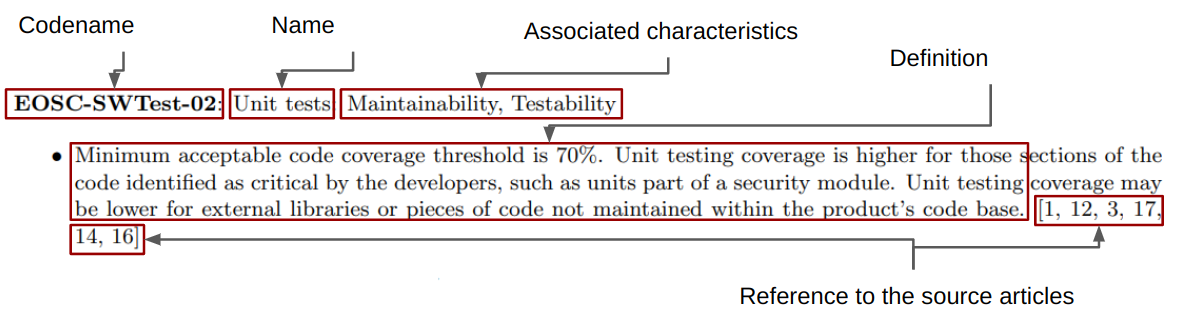
\includegraphics[width=0.9\linewidth]{../imgs/qa.png}
    \caption{The structure of each Attribute or Metric entry.}
    \label{fig:sqattr}
\end{figure}

\newpage
\subsection{Source Code Metrics: EOSC-SCMet}

\textbf{EOSC-SCMet-01}: Size of the software application: Maintainability.

\begin{itemize}
    \item The software product's rebuild value is estimated from the number of lines of code. This value is calculated in man-years using the Programming Languages Table of the Software Productivity Research Software Productivity Research \cite{baggen_standardized_2012}.
\end{itemize}

\textbf{EOSC-SCMet-02}: \% of redundant code: Maintainability, Modifiability.

\begin{itemize}
    \item A line of code is considered redundant if it is part of a code fragment (larger than 6 lines of code) that is repeated literally (modulo white-space) in at least one other location in the source code \cite{baggen_standardized_2012}.
\end{itemize}

\textbf{EOSC-SCMet-03}: \# Lines of code: Maintainability.

\begin{itemize}
    \item Number of lines for the whole software project or components / modules / classes / functions / methods \cite{montagud_systematic_2012,baggen_standardized_2012}.
\end{itemize}

\textbf{EOSC-SCMet-04}: \% of assertions: Maintainability.

\begin{itemize}
    \item Percentage of lines of source code containing assertions. Assertions are used as a means for demonstrating that the program is behaving as expected and as an indication of how thoroughly the source classes have been tested on a per class level \cite{nagappan_early_2005}.
\end{itemize}

\textbf{EOSC-SCMet-05}: Cyclomatic Complexity: Maintainability.

\begin{itemize}
    \item Cyclomatic complexity (i.e.,  the number of linearly independent paths through a program's source code) of the whole software component or modules/components/classes/functions/methods. Cyclomatic complexity is created by calculating the number of different code paths in the flow of the program. A program that has complex control flow requires more tests to achieve good code coverage and is less maintainable \cite{srisopha_software_2018,montagud_systematic_2012,baggen_standardized_2012,nagappan_early_2005,ogasawara_experiences_1996}.
\end{itemize}

\textbf{EOSC-SCMet-06}: Cyclomatic Complexity test/source ratio: Maintainability.

\begin{itemize}
    \item Ratio between the sum of cyclomatic complexities of all tests and the source code \cite{nagappan_early_2005}.
\end{itemize}

\textbf{EOSC-SCMet-07}: Number of arguments: Maintainability.

\begin{itemize}
    \item Number of arguments or parameters used in functions. Functions with many parameters may be a symptom of bad encapsulation \cite{baggen_standardized_2012,ogasawara_experiences_1996}.
\end{itemize}

\textbf{EOSC-SCMet-08}: Number of function calls: Maintainability.

\begin{itemize}
    \item Measures the interdependencies between unique classes through parameters, local variables, return types, method calls, generic or template instantiations, base classes, interface implementations, fields defined on external types, and attribute decoration. Good software design dictates that types and methods should have high cohesion and low coupling. High coupling indicates a design that is difficult to reuse and maintain because of its many interdependencies on other types \cite{montagud_systematic_2012,ogasawara_experiences_1996}.
\end{itemize}

\textbf{EOSC-SCMet-09}: Modularity: Maintainability, Functional suitability.

\begin{itemize}
    \item Degree to which a system or computer program is composed of discrete components such that a change to one component has minimal impact on other components. Also the number of modules \cite{iso_25010_2011_2017,montagud_systematic_2012,aberdour_achieving_2007,ogasawara_experiences_1996,shepherdson_cessda_2019}.
\end{itemize}

\textbf{EOSC-SCMet-10}: Number of comments: Modifiability.

\begin{itemize}
    \item Number of lines corresponding to comments for the whole software or per modules/components / classes / functions / methods \cite{srisopha_software_2018,montagud_systematic_2012,ogasawara_experiences_1996}.
\end{itemize}

\textbf{EOSC-SCMet-11}: Maintainability Index (MI): Maintainability.

\begin{itemize}
    \item Degree of effectiveness and efficiency with which a product or system can be modified by the intended maintainers. The Maintainability Index (MI) calculates an index value between 0 and 100 that represents the relative ease of maintaining the code. A high value means better maintainability. Colour coded ratings can be used to quickly identify trouble spots in the code. A green rating is between 20 and 100 and indicates that the code has good maintainability. A yellow rating is between 10 and 19 and indicates that the code is moderately maintainable. A red rating is a rating between 0 and 9 \cite{iso_25010_2011_2017,montagud_systematic_2012}.
\end{itemize}

\textbf{EOSC-SCMet-12}: Internal cohesion: Maintainability.

\begin{itemize}
    \item Cohesion describes how related the functions within a single module are. Low cohesion implies that a given module performs tasks which are not very related to each other and hence can create problems as the module becomes large \cite{iso_iec_24765_2017,montagud_systematic_2012}.
\end{itemize}

\textbf{EOSC-SCMet-13}: Test class to source class ratio: Reliability.

\begin{itemize}
    \item Control measure to counter the confounding effect of class size. The coefficient is calculated by TLOC+/SLOC  (TLOC = number of test classes, SLOC = number of source classes) \cite{nagappan_early_2005}.
\end{itemize}

\textbf{EOSC-SCMet-14}: Coupling Between Objects (CBO) ratio: Maintainability.

\begin{itemize}
    \item Ratio between the CBO in the tests and in the whole source code. The higher the inter-object class coupling, the more rigorous the testing should be \cite{nagappan_early_2005}.
\end{itemize}

\textbf{EOSC-SCMet-15}: Depth of inheritance Tree (DIT) ratio: Maintainability.

\begin{itemize}
    \item Ratio between the DIT of the tests and the DIT of the source code. A higher DIT indicates desirable reuse but adds to the complexity of the code because a change or a failure in a super class propagates down the inheritance tree \cite{nagappan_early_2005}.
\end{itemize}

\textbf{EOSC-SCMet-16}: Weighted Methods per Class (WMC) ratio: Maintainability.

\begin{itemize}
    \item Ratio between the WMC of the tests with respect to the WMC of the whole source code. This measure serves to compare the testing effort on a method basis. WMC is an indicator of fault-proneness \cite{nagappan_early_2005}.
\end{itemize}

\textbf{EOSC-SCMet-17}: Source lines of code (SLOC) ratio: Maintainability.

\begin{itemize}
    \item SLOC of the whole project with respect to the minimum SLOC of its components \cite{nagappan_early_2005}.
\end{itemize}

% \mdavid This is basically modularity EOSC-SCMet-09 already referenced there
% \textbf{EOSC-SCMet-18}: Number of include files: Maintainability.

% \begin{itemize}
%     \item Number of imported modules \cite{ogasawara_experiences_1996}.
% \end{itemize}

% \mdavid This is Cyclomatic complexity, will be reference there
% \textbf{EOSC-SCMet-19}: Number of conditions per module: Maintainability.

% \begin{itemize}
%     \item Number of conditions per module \cite{ogasawara_experiences_1996}.
% \end{itemize}

% \textbf{EOSC-SCMet-20}: Number of loops per module: Maintainability.

% \begin{itemize}
%     \item Number of loops per module \cite{ogasawara_experiences_1996}.
% \end{itemize}

\subsection{Time and Performance Metrics: EOSC-TMet}

\textbf{EOSC-TMet-01}: Effort required for changes: Reliability, Supportability.

\begin{itemize}
    \item Time and resources dedicated to resolve an issue \cite{montagud_systematic_2012}.
\end{itemize}

\textbf{EOSC-TMet-02}: \# Resolved bugs: Supportability.

\begin{itemize}
    \item Number of resolved bugs per period of time \cite{montagud_systematic_2012}.
\end{itemize}

\textbf{EOSC-TMet-03}: \# Open bugs: Supportability.

\begin{itemize}
    \item Number of open bugs/issues per period of time \cite{montagud_systematic_2012}.
\end{itemize}

\textbf{EOSC-TMet-04}: Defect rates: Maintainability.

\begin{itemize}
    \item The number of outstanding defects in a product per period of time \cite{crispin_driving_2006}.
\end{itemize}

\textbf{EOSC-TMet-05}: Integrity: Integrity, Maintainability.

\begin{itemize}
    \item Resource cost expended to solve problems caused by inconsistencies within the system. This may be measured in terms of staff time employed to fix problems and user time wasted. Also, degree to which a system, product or component prevents unauthorised access to, or modification of, computer programs or data \cite{iso_25010_2011_2017,gillies_modelling_1992}.
\end{itemize}

\textbf{EOSC-TMet-06}: Maintainability: Maintainability.

\begin{itemize}
    \item Measured by the resources spent in terms of time and cost in keeping a system up and running over a period of time \cite{gillies_modelling_1992,boehm_quantitative_1976}.
\end{itemize}

\textbf{EOSC-TMet-07}: Adaptability: Reusability. Adaptability.

\begin{itemize}
    \item Degree to which a product or system can effectively and efficiently be adapted for different or evolving hardware, software or other operational or usage environments \cite{iso_25010_2011_2017,gillies_modelling_1992,boehm_quantitative_1976}.
\end{itemize}

\textbf{EOSC-TMet-08}: \# Registered users: Operability.

\begin{itemize}
    \item The metric Number of registered users is to be collected \cite{orviz_fernandez_eosc-synergy_2020}.
\end{itemize}

\textbf{EOSC-TMet-09}: \# Active users: Operability.

\begin{itemize}
    \item The metric Number of active users over a given period of time may be collected \cite{orviz_fernandez_eosc-synergy_2020}.
\end{itemize}

\textbf{EOSC-TMet-10}: Amount of computing resources: Operability, Performance Efficiency.

\begin{itemize}
    \item The metric amount of computing resources per user or group of users is collected. An example is CPU x hours, resource utilisation \cite{iso_25010_2011_2017,orviz_fernandez_eosc-synergy_2020}.
\end{itemize}

\textbf{EOSC-TMet-11}: Amount of storage resources: Operability, Performance Efficiency.

\begin{itemize}
    \item The metric amount of storage resources per user or group of users is collected. An example is GByte x hours. Resource utilisation and capacity \cite{iso_25010_2011_2017,orviz_fernandez_eosc-synergy_2020}.
\end{itemize}

\subsection{Qualitative Attributes: EOSC-Qual}

\textbf{EOSC-Qual-01}: Complexity of diagrams: Maintainability. Reusability.

\begin{itemize}
    \item Complexity of diagrams (UML) for the whole software or modules/components \cite{montagud_systematic_2012}.
\end{itemize}

\textbf{EOSC-Qual-02}: Complexity of architecture: Maintainability. Reusability.

\begin{itemize}
    \item Architecture showing modules and interactions \cite{montagud_systematic_2012,zuser_software_2005}.
\end{itemize}

\textbf{EOSC-Qual-03}: Complexity of a use case: Maintainability. Reusability. Usability.

\begin{itemize}
    \item Complexity of use case diagrams (UML) \cite{montagud_systematic_2012}.
\end{itemize}

\textbf{EOSC-Qual-04}: Sustainable community: Supportability.

\begin{itemize}
    \item An active community is behind the software product \cite{aberdour_achieving_2007}.
\end{itemize}

\textbf{EOSC-Qual-05}: User satisfaction: Attractiveness.

\begin{itemize}
    \item Degree to which a user interface enables pleasing and satisfying interaction for the user \cite{iso_25010_2011_2017,zuser_software_2005}.
\end{itemize}

\textbf{EOSC-Qual-06}: Usability: Usability.

\begin{itemize}
    \item Measured using user surveys. However, it may also be assessed in terms of calls upon support staff, e.g. number of requests for help or support staff time expended. Also, degree to which a product or system can be used by specified users to achieve specific goals with effectiveness, efficiency and satisfaction in a specified context of use \cite{iso_25010_2011_2017,zuser_software_2005,gillies_modelling_1992,boehm_quantitative_1976}.
\end{itemize}

\textbf{EOSC-Qual-07}: Reliability: Reliability.

\begin{itemize}
    \item The reliability of systems from the user's point of view is concerned with three things: (1) How often does it go wrong? (2) How long is it unavailable? (3) Is any information lost at recovery? Also, degree to which a system, product or component performs specific functions under specified conditions for a specified period of time \cite{iso_25010_2011_2017,gillies_modelling_1992,boehm_quantitative_1976}.
\end{itemize}

\textbf{EOSC-Qual-08}: Portability: Portability.

\begin{itemize}
    \item Degree of effectiveness and efficiency with which a system, product or component can be transferred from one hardware, software or other operational or usage environment to another \cite{iso_25010_2011_2017,gillies_modelling_1992,boehm_quantitative_1976,shepherdson_cessda_2019,raymond_software_2013}.
\end{itemize}

\textbf{EOSC-Qual-09}: Timeliness: Supportability.

\begin{itemize}
    \item Assessed in terms of the costs of non-delivery. These will possibly include staff time and lost sales. It may also be assessed in terms of the number of days departure from the date agreed with client \cite{gillies_modelling_1992}.
\end{itemize}

\textbf{EOSC-Qual-10}: Cost-Benefit efficiency: Maintainability.

\begin{itemize}
    \item Measured in simple financial terms. The costs of installing and maintaining the system are weighed against the assessment of business benefits \cite{gillies_modelling_1992}.
\end{itemize}

\textbf{EOSC-Qual-11}: Accessibility: Technical accessibility.

\begin{itemize}
    \item Degree to which a product or system can be used by people with the widest range of characteristics and capabilities to achieve a specified goal in a specified context of use \cite{iso_25010_2011_2017,boehm_quantitative_1976}.
\end{itemize}

\textbf{EOSC-Qual-12}: Accountability: Performance, Resource utilisation.

\begin{itemize}
    \item Degree to which the actions of an entity can be traced uniquely to the entity. Its usage can be measured; critical segments of code can be instrumented with probes to measure timing, whether specified branches are exercised, etc. \cite{iso_25010_2011_2017,boehm_quantitative_1976}.
\end{itemize}

\textbf{EOSC-Qual-13}: Accuracy: Performance, Functional suitability.

\begin{itemize}
    \item Code outputs are sufficiently precise to satisfy their intended use \cite{boehm_quantitative_1976}.
\end{itemize}

\textbf{EOSC-Qual-14}: Communicativeness: Ease of use.

\begin{itemize}
    \item Metric which facilitates the specification of inputs and provides outputs whose form and content are easy to assimilate and useful \cite{boehm_quantitative_1976,raymond_software_2013}.
\end{itemize}

\textbf{EOSC-Qual-15}: Completeness: Supportability, Manageability.

\begin{itemize}
    \item All software parts are present and each part is fully developed \cite{iso_25010_2011_2017,boehm_quantitative_1976}.
\end{itemize}

\textbf{EOSC-Qual-16}: Conciseness: Supportability, Resource utilisation.

\begin{itemize}
    \item Redundant information about the software code is not present \cite{boehm_quantitative_1976}.
\end{itemize}

\textbf{EOSC-Qual-17}: Consistency: Maintainability, Interoperability, Compatibility.

\begin{itemize}
    \item Source code contains uniform notation, terminology and symbology within itself \cite{boehm_quantitative_1976,raymond_software_2013}.
\end{itemize}

\textbf{EOSC-Qual-18}: Legibility: Supportability, Maintainability.

\begin{itemize}
    \item Software function is easily discerned by reading the code \cite{boehm_quantitative_1976}.
\end{itemize}

\textbf{EOSC-Qual-19}: Modifiability: Modifiability.

\begin{itemize}
    \item Degree to which a product or system can be effectively and efficiently modified without introducing defects or degrading existing product quality \cite{iso_25010_2011_2017,boehm_quantitative_1976}.
\end{itemize}

\textbf{EOSC-Qual-20}: Robustness: Safety.

\begin{itemize}
    \item Software can continue to perform despite some violation of the assumptions in its specification \cite{boehm_quantitative_1976}.
\end{itemize}

\textbf{EOSC-Qual-21}: Self-containedness: Supportability.

\begin{itemize}
    \item Software performs all its explicit and implicit functions within itself \cite{boehm_quantitative_1976}.
\end{itemize}

\textbf{EOSC-Qual-22}: Self-descriptiveness: Supportability, Ease of use.

\begin{itemize}
    \item Software contains enough information for a reader to determine or verify its objectives, assumptions, constraints, inputs, outputs, components, and revision status \cite{boehm_quantitative_1976}.
\end{itemize}

\textbf{EOSC-Qual-23}: Structuredness: Modifiability, Reusability.

\begin{itemize}
    \item Software possesses a definite pattern of organisation of its interdependent parts \cite{boehm_quantitative_1976}.
\end{itemize}

\textbf{EOSC-Qual-24}: Understandability: Supportability.

\begin{itemize}
    \item Software purpose is clear to the inspector \cite{boehm_quantitative_1976}.
\end{itemize}

\textbf{EOSC-Qual-25}: Intellectual Property: Supportability, Reusability.

\begin{itemize}
    \item There are multiple statements embedded into the software product describing unrestricted rights and any conditions for use, including commercial and non-commercial use, and the recommended citation. The list of developers is embedded in the source code of the product, in the documentation, and in the expression of the software upon execution. The intellectual property rights statements are expressed in legal language, machine-readable code, and in concise statements in language that can be understood by laypersons, such as a pre-written, recognizable licence \cite{shepherdson_cessda_2019}.
\end{itemize}

\textbf{EOSC-Qual-26}: Extensibility: Attractiveness, Modifiability.

\begin{itemize}
    \item There is evidence that the software project has been extended externally by users outside of the original development group using existing documentation only. There is a clear approach for modifying and extending features across and in multiple scenarios, with specific documentation and features to allow the building of extensions which are used across a range of domains by multiple user groups. There may be a library available of user-generated content for extensions and user generated documentation on extension is also available \cite{shepherdson_cessda_2019}.
\end{itemize}

\textbf{EOSC-Qual-27}: Standards compliance: Functional suitability.

\begin{itemize}
    \item Compliance with open or internationally recognized standards for the software and software development process, is evident and documented, and verified through testing of all components. Ideally independent verification is documented through regular testing and certification from an independent group \cite{shepherdson_cessda_2019}.
\end{itemize}

\textbf{EOSC-Qual-28}: Internationalisation and localization: Usability.

\begin{itemize}
    \item Demonstrable usability: Software has been tested with multiple pseudo or genuine translations \cite{shepherdson_cessda_2019}.
\end{itemize}

\subsection{DevOps-SW Release and Management Attributes: EOSC-SWRelMan}

\textbf{EOSC-SWRelMan-01}: Open source : Supportability, Maintainability, Availability, Reusability.

\begin{itemize}
    \item Following the open-source model, the source code being produced is open and publicly available to promote the adoption and augment the visibility of the software developments \cite{orviz_set_2017,raymond_software_2013}.
\end{itemize}

\textbf{EOSC-SWRelMan-02}: Version Control System (VCS): Supportability, Maintainability.

\begin{itemize}
    \item Source code uses a Version Control System (VCS). All software components delivered by the same project agree on a common VCS \cite{orviz_set_2017}.
\end{itemize}

\textbf{EOSC-SWRelMan-03}: Source code hosting: Supportability, Maintainability.

\begin{itemize}
    \item Source code produced within the scope of a broader development project resides in a common organisation of a version control repository hosting service \cite{orviz_set_2017}.
\end{itemize}

\textbf{EOSC-SWRelMan-04}: Working state version: Maintainability.

\begin{itemize}
    \item The main branch in the source code repository maintains a working state version of the software component. Main branch is protected to disallow force pushing, thus preventing untested and un-reviewed source code from entering the production-ready version. New features are merged in the main branch whenever the agreed upon SQA criteria is fulfilled \cite{orviz_set_2017}.
\end{itemize}

\textbf{EOSC-SWRelMan-05}: Changes branches: Maintainability.

\begin{itemize}
    \item New changes in the source code are placed in individual branches. Branches follow a common nomenclature, usually by prefixing, to differentiate change types (e.g. feature, release, fix) \cite{orviz_set_2017}.
\end{itemize}

\textbf{EOSC-SWRelMan-06}: Good patching practice: Maintainability.

\begin{itemize}
    \item Secondary long-term branch that contains the changes for the next software release exists. Next release changes come from the individual branches. Once ready for release, changes in the secondary long-term branch are merged into the main branch and versioned. At that point in time, main and secondary branches are aligned. This step marks a production release \cite{orviz_set_2017,raymond_software_2013}.
\end{itemize}

\textbf{EOSC-SWRelMan-07}: Support: Maintainability, Operability.

\begin{itemize}
    \item Existence of an issue tracking system or helpdesk, facilitates structured software development. Leveraging issues to track down both new enhancements and defects (bugs, documentation typos). Applies as well to services to report operational and user issues \cite{srisopha_software_2018,shepherdson_cessda_2019,orviz_set_2017,orviz_fernandez_eosc-synergy_2020}.
\end{itemize}

\textbf{EOSC-SWRelMan-08}: Code review: Maintainability.

\begin{itemize}
    \item Code reviews are done in the agreed peer review tool within the project, with the following  functionality: (a) Allows general and specific comments on the line or lines that need to be reviewed. (b) Shows the results of the required change-based test executions. (c) Allows to prevent merges of the candidate change whenever not all the required tests are successful. Exceptions to this rule cover the third-party or upstream contributions which MAY use the existing mechanisms or tools for code review provided by the target software project. This exception is only allowed whenever the external revision lifecycle does not interfere with the project deadlines \cite{srisopha_software_2018,aberdour_achieving_2007,zuser_software_2005,orviz_set_2017}.
\end{itemize}

\textbf{EOSC-SWRelMan-09}: Semantic Versioning : Maintainability.

\begin{itemize}
    \item Semantic Versioning specification is followed for tagging the production releases \cite{orviz_set_2017,raymond_software_2013}.
\end{itemize}

\textbf{EOSC-SWRelMan-10}: Open-source licence: Supportability, Maintainability, Reusability.

\begin{itemize}
    \item As open-source software, source code adheres to an open-source licence to be freely used, modified and distributed by others. Non-licensed software is exclusive copyright by default \cite{orviz_set_2017,raymond_software_2013}.
\end{itemize}

\textbf{EOSC-SWRelMan-11}: Metadata: Supportability, Maintainability, Availability.

\begin{itemize}
    \item A metadata file (such as Codemeta or Citation File Format) exists alongside the code, under its VCS. The metadata file is updated when needed, as is the case of a new version \cite{orviz_set_2017}.
\end{itemize}

\textbf{EOSC-SWRelMan-12}: Packaging: Installability.

\begin{itemize}
    \item Production-ready code is  built as an artifact that can be installed on a system \cite{shepherdson_cessda_2019,orviz_set_2017,raymond_software_2013}.
\end{itemize}

\textbf{EOSC-SWRelMan-13}: Register/publish artifact: Installability.

\begin{itemize}
    \item The built artifact is uploaded and registered into a public repository of such artefacts \cite{orviz_set_2017}.
\end{itemize}

\textbf{EOSC-SWRelMan-14}: Notification upon registration: Installability.

\begin{itemize}
    \item Upon success of the package delivery process, a notification is sent to pre-defined parties such as the main developer or team \cite{orviz_set_2017}.
\end{itemize}

\textbf{EOSC-SWRelMan-15}: Code deployment: Installability.

\begin{itemize}
    \item Production-ready code is deployed as a workable system with the minimal user or system administrator interaction leveraging software configuration management (SCM) tools \cite{orviz_set_2017}.
\end{itemize}

\textbf{EOSC-SWRelMan-16}: Software Configuration Management (SCM) as code: Installability.

\begin{itemize}
    \item A software configuration management (SCM) module is treated as code. Version controlled, it resides in a different repository than the source code to facilitate the distribution \cite{orviz_set_2017}.
\end{itemize}

\textbf{EOSC-SWRelMan-17}: SCM tool: Installability.

\begin{itemize}
    \item All software components delivered by the same project agree on a common SCM tool. However, software products are not restricted to provide a unique solution for the automated deployment \cite{orviz_set_2017}.
\end{itemize}

\textbf{EOSC-SWRelMan-18}: SCM code changes: Installability.

\begin{itemize}
    \item Any change affecting the applications deployment or operation is subsequently reflected in the relevant SCM modules \cite{orviz_set_2017}.
\end{itemize}

\textbf{EOSC-SWRelMan-19}: SCM official repositories: Installability.

\begin{itemize}
    \item Official repositories provided by the manufacturer are used to host the SCM modules, thus augmenting the visibility and promote external collaboration \cite{orviz_set_2017}.
\end{itemize}

\textbf{EOSC-SWRelMan-20}: Installability: Installability.

\begin{itemize}
    \item Degree of effectiveness and efficiency with which a product or system can be successfully installed and/or uninstalled in a specified environment. Also, a production-ready SW or service is deployed as a workable system with the minimal user or system administrator interaction leveraging Infrastructure as Code templates \cite{iso_25010_2011_2017,orviz_fernandez_eosc-synergy_2020}.
\end{itemize}

\textbf{EOSC-SWRelMan-21}: Preserve immutable infrastructures: Installability.

\begin{itemize}
    \item Any future change to a deployed Service is done in the form of a new deployment, in order to preserve immutable infrastructures \cite{orviz_fernandez_eosc-synergy_2020}.
\end{itemize}

\textbf{EOSC-SWRelMan-22}: Infrastructure as Code (IaC) validation: Installability.

\begin{itemize}
    \item IaC is validated by specific (unit) testing frameworks for every change being done \cite{orviz_fernandez_eosc-synergy_2020}.
\end{itemize}

\textbf{EOSC-SWRelMan-23}: Packaging of tarballs: Installability.

\begin{itemize}
    \item Tarballs are not included in the distribution directory. Packaged tarballs are not extracted in the distribution directory \cite{raymond_software_2013}.
\end{itemize}

\textbf{EOSC-SWRelMan-24}: Design for upgradability: Compatibility.

\begin{itemize}
    \item Installation layout supports different versions and code releases \cite{raymond_software_2013}.
\end{itemize}

\textbf{EOSC-SWRelMan-25}: Provide checksums: Maintainability.

\begin{itemize}
    \item Code releases provide checksums with each binary (tarballs, RPMs, etc.) \cite{raymond_software_2013}.
\end{itemize}

\textbf{EOSC-SWRelMan-26}: Documentation version controlled: Supportability.

\begin{itemize}
    \item Documentation is version controlled. \cite{orviz_fernandez_eosc-synergy_2020}.
\end{itemize}

\textbf{EOSC-SWRelMan-27}: Documentation as code: Supportability, Maintainability, Reusability.

\begin{itemize}
    \item Documentation is treated as code and resides in the same repository where the source code lies \cite{orviz_set_2017}.
\end{itemize}

\textbf{EOSC-SWRelMan-28}: Documentation formats: Supportability, Maintainability, Reusability.

\begin{itemize}
    \item Documentation uses plain text format using a markup language, such as Markdown or reStructuredText. All software components delivered by the same project agree on a common markup language \cite{orviz_set_2017,raymond_software_2013}.
\end{itemize}

\textbf{EOSC-SWRelMan-29}: Documentation online: Supportability, Availability.

\begin{itemize}
    \item Documentation is online available in a documentation repository. Documentation is rendered automatically \cite{orviz_set_2017,orviz_fernandez_eosc-synergy_2020}.
\end{itemize}

\textbf{EOSC-SWRelMan-30}: Documentation updates: Supportability, Maintainability, Reusability.

\begin{itemize}
    \item Documentation is updated on new software or service versions involving any substantial or minimal change in the behaviour of the application \cite{orviz_set_2017,orviz_fernandez_eosc-synergy_2020,raymond_software_2013}.
\end{itemize}

\textbf{EOSC-SWRelMan-31}: Documentation updates if inaccurate/unclear: Supportability, Maintainability, Reusability.

\begin{itemize}
    \item Documentation is updated whenever reported as inaccurate or unclear \cite{orviz_set_2017,orviz_fernandez_eosc-synergy_2020}.
\end{itemize}

\textbf{EOSC-SWRelMan-32}: Documentation production: Supportability, Maintainability, Reusability.

\begin{itemize}
    \item Documentation is produced according to the target audience, varying according to the software component specification. The identified types of documentation and their content are README file(one-paragraph description of the application, a "Getting Started" step-by-step description on how to get a development environment running, automated test execution how-to, links to external documentation below, contributing code of conduct, versioning specification, author list and contacts, licence information and acknowledgements), Developer documentations (Private API documentation, structure and interfaces and build documentation), Deployment and Administration documentations (Installation and configuration guides, service reference card, FAQs and troubleshooting) and user documentations (Public API documentation and command-line reference) \cite{aberdour_achieving_2007,shepherdson_cessda_2019,orviz_set_2017,orviz_fernandez_eosc-synergy_2020,raymond_software_2013}.
\end{itemize}

\textbf{EOSC-SWRelMan-33}: Documentation PID: Supportability.

\begin{itemize}
    \item Documentation has a Persistent Identifier (PID) \cite{orviz_fernandez_eosc-synergy_2020}.
\end{itemize}

\textbf{EOSC-SWRelMan-34}: Documentation licence: Supportability.

\begin{itemize}
    \item Documentation has a non-software licence \cite{orviz_fernandez_eosc-synergy_2020}.
\end{itemize}

\subsection{DevOps - Testing Attributes: EOSC-SWTest}

\textbf{EOSC-SWTest-01}: Code style: Maintainability, Testability.

\begin{itemize}
    \item Each individual software complies with a de-facto code style standard for all the programming languages used in the codebase. Multiple standard style compliance is possible \cite{orviz_set_2017,raymond_software_2013}.
\end{itemize}

\textbf{EOSC-SWTest-02}: Unit tests: Maintainability, Testability.

\begin{itemize}
    \item Minimum acceptable code coverage threshold is 70\%. Unit testing coverage is higher for those sections of the code identified as critical by the developers, such as units part of a security module. Unit testing coverage may be lower for external libraries or pieces of code not maintained within the product's code base \cite{aberdour_achieving_2007,nagappan_early_2005,boehm_quantitative_1976,shepherdson_cessda_2019,orviz_set_2017,raymond_software_2013}.
\end{itemize}

\textbf{EOSC-SWTest-03}: Test doubles: Functional suitability, Testability.

\begin{itemize}
    \item When working on automated testing,  Test Doubles (i.e., objects or procedures that look and behave like their release-intended counterparts, but are actually simplified versions that reduce the complexity and facilitate testing) are used to mimic a simplistic behaviour of objects and procedures \cite{orviz_set_2017,orviz_fernandez_eosc-synergy_2020}.
\end{itemize}

\textbf{EOSC-SWTest-04}: Test-Driven Development (TDD): Functional suitability, Maintainability, Testability.

\begin{itemize}
    \item Software requirements are converted to test cases, and these test cases are checked automatically. Also, degree of effectiveness and efficiency with which test criteria can be established for a system, product or component and tests can be performed to determine whether those criteria have been met \cite{iso_25010_2011_2017,crispin_driving_2006,zuser_software_2005,orviz_set_2017}.
\end{itemize}

\textbf{EOSC-SWTest-05}: API testing: Functional suitability, Testability.

\begin{itemize}
    \item API testing MUST cover the validation of the features outlined in the specification (aka contract testing) \cite{orviz_fernandez_eosc-synergy_2020}.
\end{itemize}

\textbf{EOSC-SWTest-06}: Integration testing: Functional suitability, Testability, Interoperability.

\begin{itemize}
    \item Whenever a new functionality is involved, integration testing guarantees the operation of any previously-working interaction with external services \cite{iso_25010_2011_2017,orviz_fernandez_eosc-synergy_2020}.
\end{itemize}

\textbf{EOSC-SWTest-07}: Functional testing: Functional suitability, Testability.

\begin{itemize}
    \item Functional testing covers the full scope -e.g. positive, negative, edge cases- for the set of functionality that the software or service claims to provide \cite{iso_25010_2011_2017,orviz_fernandez_eosc-synergy_2020}.
\end{itemize}

\textbf{EOSC-SWTest-08}: Performance testing: Functional suitability, Testability.

\begin{itemize}
    \item Performance testing is carried out to check the Software Application performance under varying loads \cite{iso_25010_2011_2017,orviz_fernandez_eosc-synergy_2020}.
\end{itemize}

\textbf{EOSC-SWTest-09}: Stress testing: Functional suitability, Testability.

\begin{itemize}
    \item Stress testing is carried out to check the Service to determine the behavioural limits under sudden increased load \cite{orviz_fernandez_eosc-synergy_2020}.
\end{itemize}

\textbf{EOSC-SWTest-10}: Scalability testing: Functional suitability, Testability.

\begin{itemize}
    \item Scalability testing is carried out to check the Service ability to scale up and/or scale out when its load reaches the limits \cite{orviz_fernandez_eosc-synergy_2020}.
\end{itemize}

\textbf{EOSC-SWTest-11}: Elasticity testing: Functional suitability, Testability.

\begin{itemize}
    \item Elasticity testing is carried out to check the Service ability to scale out or scale in, depending on its demand or workload \cite{orviz_fernandez_eosc-synergy_2020}.
\end{itemize}

\textbf{EOSC-SWTest-12}: Open Web Application Security Project (OWASP): Security.

\begin{itemize}
    \item Application is compliant with Open Web Application Security Project (OWASP) secure coding guidelines \cite{orviz_set_2017}.
\end{itemize}

\textbf{EOSC-SWTest-13}: Static Application Security Testing (SAST): Security.

\begin{itemize}
    \item Source code uses automated linter tools to perform static application security testing (SAST) that flag common suspicious constructs that may cause a bug or lead to a security risk (e.g. inconsistent data structure sizes or unused resources) \cite{orviz_set_2017}.
\end{itemize}

\textbf{EOSC-SWTest-14}: Security code reviews: Security.

\begin{itemize}
    \item Security code reviews for certain vulnerabilities is done as part of the identification of potential security flaws in the code. Inputs  come from automated linters and manual penetration testing results \cite{gillies_modelling_1992,shepherdson_cessda_2019,orviz_set_2017}.
\end{itemize}

\textbf{EOSC-SWTest-15}: No world-writable files or directories: Security.

\begin{itemize}
    \item World-writable files or directories are not present in the product's configuration or logging locations \cite{orviz_set_2017}.
\end{itemize}

\textbf{EOSC-SWTest-16}: Public endpoints and APIs encrypted: Security.

\begin{itemize}
    \item The Service public endpoints and APIs are secured with data encryption \cite{orviz_fernandez_eosc-synergy_2020}.
\end{itemize}

\textbf{EOSC-SWTest-17}: Strong ciphers: Security.

\begin{itemize}
    \item The Service uses strong ciphers for data encryption \cite{orviz_fernandez_eosc-synergy_2020}.
\end{itemize}

\textbf{EOSC-SWTest-18}: Authentication and Authorization: Security, Technical accessibility.

\begin{itemize}
    \item The Service has an authentication and authorization mechanism. The Service validates the credentials and signatures \cite{shepherdson_cessda_2019,orviz_fernandez_eosc-synergy_2020}.
\end{itemize}

\textbf{EOSC-SWTest-19}: API security assessment: Security.

\begin{itemize}
    \item API testing includes the assessment of the security-related criteria \cite{orviz_fernandez_eosc-synergy_2020}.
\end{itemize}

\textbf{EOSC-SWTest-20}: Service compliance with data regulations (GDPR): Security.

\begin{itemize}
    \item The Service handles personal data in compliance with the applicable regulations, such as the General Data Protection Regulation (GDPR) within the European boundaries \cite{orviz_fernandez_eosc-synergy_2020}.
\end{itemize}

\textbf{EOSC-SWTest-21}: Dynamic Application Security Testing (DAST): Security.

\begin{itemize}
    \item DAST checks are executed, through the use of ad-hoc tools, directly to an operational Service in order to uncover runtime security vulnerabilities and any other environment-related issues (e.g. SQL injection, cross-site scripting or DDOS). The latest release of OWASP's Web Security Testing Guide and the NIST's Technical Guide to Information Security Testing and Assessment are considered for carrying out comprehensive Service security testing \cite{orviz_fernandez_eosc-synergy_2020}.
\end{itemize}

\textbf{EOSC-SWTest-22}: Interactive Application Security Testing (IAST): Security.

\begin{itemize}
    \item Interactive Application Security Testing (IAST), analyses code for security vulnerabilities while the app is run by an automated test. IAST is performed to a service in an operating state \cite{orviz_fernandez_eosc-synergy_2020}.
\end{itemize}

\textbf{EOSC-SWTest-23}: Security penetration testing: Security.

\begin{itemize}
    \item Penetration testing (manual or automated) is part of the application security verification effort \cite{orviz_fernandez_eosc-synergy_2020}.
\end{itemize}

\textbf{EOSC-SWTest-24}: Security assessment: Security.

\begin{itemize}
    \item The security assessment of the target system configuration is particularly important to reduce the risk of security attacks. The benchmarks delivered by the Center for Internet Security (CIS) and the NIST's Security Assurance Requirements for Linux Application Container Deployments are considered for this task. Also, the degree to which a product or system protects information and data so that persons or other products or systems have the degree of data access appropriate to their types and levels of authorization \cite{iso_25010_2011_2017,orviz_fernandez_eosc-synergy_2020}.
\end{itemize}

\textbf{EOSC-SWTest-25}: Security as Code (SaC) Testing: Security.

\begin{itemize}
    \item IaC testing covers the security auditing of the IaC templates (SaC) in order to assure the deployment of secured Services. For all the third-party dependencies used in the IaC templates (including all kinds of software artefacts, such as Linux packages or container-based images) \cite{orviz_fernandez_eosc-synergy_2020}.
\end{itemize}

\subsection{Service Operability Attributes: EOSC-SrvOps}

\textbf{EOSC-SrvOps-01}: Acceptable Usage Policy (AUP): Supportability.

\begin{itemize}
    \item An Acceptable Usage Policy (AUP) is declared. AUP Is a set of rules applied by the owner, creator or administrator of a network, Service or system, that restrict the ways in which the network, Service or system may be used and sets guidelines as to how it should be used. The AUP can also be referred to as: Acceptable Use Policy or Fair Use Policy \cite{orviz_fernandez_eosc-synergy_2020}.
\end{itemize}

\textbf{EOSC-SrvOps-02}: Access Policy and Terms of Use: Supportability.

\begin{itemize}
    \item An Access Policy or Terms of Use (APTU) is declared. APTU represents a binding legal contract between the users (and/or customers), and the Provider of the Service. The Access Policy mandates the users (and/or customers) access to and the use of the Provider's Service \cite{orviz_fernandez_eosc-synergy_2020}.
\end{itemize}

\textbf{EOSC-SrvOps-03}: Privacy policy: Supportability.

\begin{itemize}
    \item A Privacy Policy is declared, with a data privacy statement informing the users (and/or customers), about which personal data is collected and processed when they use and interact with the Service. It states which rights the users (and/or customers) have regarding the processing of their data \cite{orviz_fernandez_eosc-synergy_2020}.
\end{itemize}

\textbf{EOSC-SrvOps-04}: Operational Level Agreement (OLA): Supportability.

\begin{itemize}
    \item The Service includes an Operational Level Agreement (OLA) with the infrastructure where it is integrated \cite{orviz_fernandez_eosc-synergy_2020}.
\end{itemize}

\textbf{EOSC-SrvOps-05}: Service Level Agreement (SLA): Supportability.

\begin{itemize}
    \item The Service includes Service Level Agreement (SLA) with user communities \cite{orviz_fernandez_eosc-synergy_2020}.
\end{itemize}

\textbf{EOSC-SrvOps-06}: Monitoring service public endpoints: Availability, Reliability.

\begin{itemize}
    \item The Service public endpoints are monitored, such as probes measuring the http or https response time \cite{orviz_fernandez_eosc-synergy_2020}.
\end{itemize}

\textbf{EOSC-SrvOps-07}: Monitoring service public APIs: Availability, Reliability.

\begin{itemize}
    \item The Service public APIs are monitored through the use of functional tests \cite{orviz_fernandez_eosc-synergy_2020}.
\end{itemize}

\textbf{EOSC-SrvOps-08}: Monitoring service Web Interface: Availability, Reliability.

\begin{itemize}
    \item The Service Web interface is monitored, this can be accomplished through the use of automated and periodic functional tests \cite{orviz_fernandez_eosc-synergy_2020}.
\end{itemize}

\textbf{EOSC-SrvOps-09}: Monitoring security public endpoints and APIs: Availability, Reliability.

\begin{itemize}
    \item The Service is monitored for public endpoints and APIs secured and strong ciphers for encryption \cite{orviz_fernandez_eosc-synergy_2020}.
\end{itemize}

\textbf{EOSC-SrvOps-10}: Monitoring security DAST: Availability, Reliability.

\begin{itemize}
    \item The Service is monitored with DAST security checks \cite{orviz_fernandez_eosc-synergy_2020}.
\end{itemize}

\textbf{EOSC-SrvOps-11}: Infrastructure monitoring: Availability, Reliability.

\begin{itemize}
    \item The Service is monitored for infrastructure-related criteria \cite{orviz_fernandez_eosc-synergy_2020}.
\end{itemize}

\textbf{EOSC-SrvOps-12}: Monitoring with Unit tests: Availability, Reliability.

\begin{itemize}
    \item IaC (unit) tests are reused as monitoring tests, thus avoiding duplication \cite{orviz_fernandez_eosc-synergy_2020}.
\end{itemize}


\newpage
\printbibliography
\end{document}
